\subsection{Disappearance of ``Type B'' Parameter Regions}
\label{sec:minrep.adding.disapp.typeB}

\todo{small intro, then another subsubsection}

\Cref{fig:minrep.path.to.disappearance} shows diagrams depicting the borders of parameter regions of specific stable cycles.
The lower left corner of the diagrams is always in the period region with the stable cycle $P_{10}^3 \equiv \Cycle{\A^7\B^3\C^7\D^3}$, the cycles in the upper left ($\Cycle{\A^6\B^3\C^6\D^3}$), upper right ($\Cycle{\A^6\B^4\C^6\D^4}$), lower right ($\Cycle{\A^7\B^4\C^7\D^4}$), and middle ($\Cycle{\A^7\B^3\C^6\D^4}$ and $\Cycle{\A^6\B^4\C^7\D^3}$) follow.
\todo{always short form / always long form / both?}
The diagrams show the evolution of the ``type B'' parameter region along a line in the parameter space from \Cref{fig:minrep.adding1.overview.initial} ($a_L = 4, b_L = -0.5$) to \Cref{fig:minrep.adding1.overview.initial} $a_L = 1, b_L = 0.5$.
This line is given by the equation $a_L = \frac{5}{2} - 3 \cdot b_L$.

\Cref{fig:minrep.path.to.disappearance.1} shows the first change that occurs on this path to period-adding.
The ``type A'' parameter region $P_{11}^4$ does no longer overlap with the ``type A'' parameter region $P_{10}^4$.
This happens to all parameter regions $P_{x}^y$, they do no longer overlap with the parameter region $P_{x-1}^y$.
But this is only true for the left side of their overlap.
On the right side they still do overlap, as we can see from the parameter regions $P_{10}^3$ and $P_{9}1^3$ in \Cref{fig:minrep.path.to.disappearance.1}.
All other overlaps remain, but they are a lot smaller now, especially the overlaps of the ``type B'' parameter region $Q_{10}^3$ in the middle with the surrounding ``type A'' parameter regions.
In the space between the lower and upper right ``type A'' parameter regions, period adding emerges.

In the next diagram, \Cref{fig:minrep.path.to.disappearance.2}, the parameter region $P_{10}^3$ now overlaps with the parameter region $P_{10}^4$.
The new overlapping area pushes the ``type B'' parameter region to the side.
It is now smaller and only has 3 boundaries.

This overlap is completed in \Cref{fig:minrep.path.to.disappearance.3} and the ``type B'' parameter region disappears completely.
In \Cref{fig:minrep.path.to.disappearance.3}, the ``type B'' parameter region is completely replaced by the overlapping ``type A'' parameter regions $P_{10}^3$ and $P_{10}^4$.
Also the ``type A'' parameter regions $P_9^3$ and $P_{10}^4$ do not overlap anymore.
The same is true for the ``type A'' parameter regions $P_{10}^3$ and $P_{11}^4$ and we can conclude it is for all $P_x^y$ and $P_{x+1}^{y+1}$.

\Cref{fig:minrep.path.to.disappearance.3} shows the parameter region boundaries when the process is completed.
The last overlap of the ``type A'' parameter regions $P_{10}^3$ and $P_{9}^3$, and therefore all $P_x^y$ and $P_{x+1}^y$, is gone.
Only the ``type A'' parameter regions with the same period overlap and in between the ``type A'' parameter regions with different periods, there is period adding.


\begin{figure}
    \centering
    \subfloat[$a_L = 2.8, b_L = -0.1$]{
        \includegraphics[width=.5 \textwidth]{62_MinimalRepr_Adding/2D_Regions_2.8/Manual/result.png}
        \label{fig:minrep.path.to.disappearance.1}
    }
    \subfloat[$a_L = 2.725, b_L = -0.075$]{
        \includegraphics[width=.5 \textwidth]{62_MinimalRepr_Adding/2D_Regions_2.725/Manual/result.png}
        \label{fig:minrep.path.to.disappearance.2}
    } \\
    \subfloat[$a_L = 2.65, b_L = -0.05$]{
        \includegraphics[width=.5 \textwidth]{62_MinimalRepr_Adding/2D_Regions_2.65/Manual/result.png}
        \label{fig:minrep.path.to.disappearance.3}
    }
    \subfloat[$a_L = 2.5, b_L = 0$]{
        \includegraphics[width=.5 \textwidth]{62_MinimalRepr_Adding/2D_Regions_2.5/Manual/result.png}
        \label{fig:minrep.path.to.disappearance.4}
    }
    \caption{Evolution of ``type B'' parameter regions when transitioning to a period adding scenario}
    \label{fig:minrep.path.to.disappearance}
\end{figure}

\subsubsection{``Type B'' Cycles Just Before Disappearing}

Just before the ``type B'' period region disappears, at $a_L = 2.675, b_L = -0.58\overline{3}$, the cycles that exist there are extremely close to colliding with 3 different borders each.
\Cref{fig:minrep.just.before.disappearance.cobb} shows the cobweb diagram of the cycles.
Both cycles are so close to each other on branches $f_\A$ and $f_\B$, that we can't tell them apart.
Even in the vastly enhanced blowup plot in the upper left corner of the figure, both cycles are almost on top of each other.
At the boundary $d_1$ the cycles split, because of the symmetry the same happens at $d_3$ again.
At $d_1$, the cycle $\Cycle{\A^7\B^3\C^6\D^4}$ (green) is mapped onto $f_\A$ one last time, while its twin cycle $\Cycle{\A^6\B^4\C^7\D^3}$ (brown) is directly mapped to $f_\B$.
At $d_3$, the same thing happens, but the two cycles are swapped.

As for the cycles near $d_0$ and $d_2$, the cycle $\Cycle{\A^7\B^3\C^6\D^4}$ is next to $d_2$, while its twin cycle is near $d_0$.
The collision of the cycles with the borders at the same time corresponds to the right boundary of the ``type B'' period region.
This follows from \Cref{sec:minrep.bif}, where all bifurcations in this model are listed and explained.
The two bifurcations are denoted as $\BCB_{d_0}^{\A^6\B^4\C^7\D^3, r}$ and $\BCB_{d_2}^{\A^7\B^3\C^6\D^4, r}$.
As this boundary does not move as much as the other two still existing boundaries when transitioning to the period adding scenario, this bifurcation is not as important to us now.

The cycles near $d_1$ and $d_3$ correspond to the upper and lower boundaries of the ``type B'' period region.
Again, the correspondence follows from \Cref{sec:minrep.bif}.
The upper and lower boundaries of ``type B'' period regions are border collision bifurcations where the two cycles collide with $d_1$ and $d_3$ at the same time, one cycle with one boundary each.
For the upper boundary, the cycle with more points on the branch $f_\A$ collides with the border $d_3$ from the left, denoted as $\BCB_{d_3}^{\A^7\B^3\C^6\D^4, l}$.
Its twin cycle collides with $d_1$, also from the left.
This follows from the symmetry and is denoted as $\BCB_{d_1}^{\A^6\B^4\C^7\D^3, l}$.
For the lower boundary, now the cycles collide from the right instead of the left, but the borders with which each cycle collides stay the same.
So for this boundary we have the bifurcations $\BCB_{d_3}^{\A^7\B^3\C^6\D^4, l}$ and $\BCB_{d_1}^{\A^6\B^4\C^7\D^3, r}$.
These two boundaries get closer to each other as we lower $a_L$ as we can see in \Cref{sec:minrep.adding.disapp.typeB}.

\begin{figure}
    \centering
    \subfloat[Regions]{
        \includegraphics[width=.3 \textwidth]{62_MinimalRepr_Adding/2D_Regions_2.675/Manual/result.png}
        \label{fig:minrep.just.before.disappearance.reg}
    }
    \subfloat[Cobweb at point $A$]{
        \includegraphics[width=.3 \textwidth]{62_MinimalRepr_Adding/Cob_2.675_A/Manual/result.png}
        \label{fig:minrep.just.before.disappearance.coba}
    }
    \subfloat[Cobweb at point $B$]{
        \includegraphics[width=.3 \textwidth]{62_MinimalRepr_Adding/Cob_2.675_B/Manual/result.png}
        \label{fig:minrep.just.before.disappearance.cobb}
    }
    \label{fig:minrep.just.before.disappearance}
    \caption{Disappearance of the ``type B'' parameter region}
\end{figure}

To see what happens after the boundaries of the ``type B'' period region crossed each other, we take a look at point $A$.
\Cref{fig:minrep.just.before.disappearance.coba} shows the cobweb diagram at this point.
The two cycles that exist here look similar to the cycles in \Cref{fig:minrep.just.before.disappearance.cobb}, they have a similar number of points on each branch.
Also, two cycles are near borders $d_1$ and $d_3$, one on the left and one on the right, as well as one cycle being near $d_0$ and $d_2$.
But with this cobweb diagram, the basins of attraction on the right half are not the inverse of the basins of attraction on the left half, but the same.
This hints at the fact that we are now dealing with ``type A'' cycles that are symmetric.

\todo{order of left most cycle and other cycle => type B or type A}

\todo{parallels to next appearing period adding}